\documentclass{book}
\usepackage[landscape,a3paper,left=0.5cm,right=1in,top=1in,bottom=1in]{geometry}
\usepackage{amsmath}
\usepackage{xcolor}
\usepackage{tikz}
\usepackage{pgfplots}
\usepackage{booktabs}
\usepackage{multirow}
\usepackage{amsmath,amssymb}

\begin{document}

\vspace{2cm}

\begin{center}\underline{\textsc{Equiv + Permut} for Test of 99 small instances of knapsack}
\vspace{0.5cm}

\begin{tabular}{ccc} & gecode & coinbc\\\\\tikz{\node (a) at (0.0,4) {\textsc{QuadraMod}};\node (a) at (0.0,0) {};} & 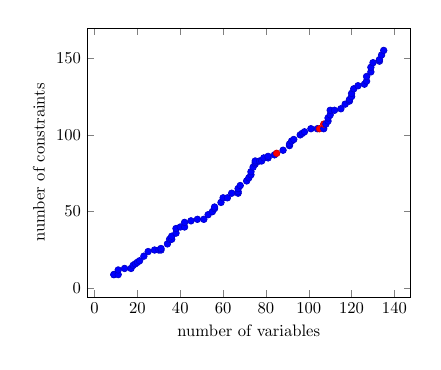
\begin{tikzpicture}[scale=0.6]
\begin{axis}[scatter, point meta=\thisrow{time}, only marks, colorbar, colorbar horizontal,colorbar style={ylabel={Time (min)}, ylabel style={rotate=270},}, colorbar to name={storedcolorbar1},, xlabel=number of variables,ylabel=number of constraints]

\addplot table[x=x,y=y]  { 
 x y time
 9 9 0.05 
 9 9 0.0 
 11 9 0.0 
 11 12 0.0 
 14 13 0.0 
 17 13 0.0 
 18 15 0.0 
 19 16 0.0 
 20 17 0.0 
 21 18 0.0 
 23 21 0.0 
 25 24 0.0 
 28 25 0.0 
 30 25 0.0 
 31 25 0.0 
 31 26 0.0 
 34 29 0.0 
 35 32 0.0 
 36 32 0.0 
 36 34 0.0 
 38 36 0.0 
 38 39 0.0 
 40 40 0.0 
 42 40 0.0 
 42 43 0.0 
 45 44 0.0 
 48 45 0.0 
 51 45 0.0 
 53 48 0.0 
 55 50 0.0 
 56 52 0.0 
 56 53 0.0 
 59 56 0.0 
 60 59 0.0 
 62 59 0.0 
 64 62 0.0 
 67 62 0.0 
 67 63 0.0 
 67 65 0.0 
 68 67 0.0 
 71 70 0.0 
 72 72 0.0 
 73 74 0.0 
 73 76 0.0 
 74 79 0.0 
 75 81 0.0 
 75 82 0.0 
 75 83 0.0 
 77 83 0.0 
 78 83 0.0 
 79 85 0.0 
 81 85 0.0 
 81 86 0.0 
 84 87 0.0 
 85 88 1440.0 
 88 90 1.0 
 91 93 1.0 
 91 94 1.0 
 92 96 1.0 
 93 97 1.0 
 96 100 1.0 
 97 101 1.0 
 98 102 1.0 
 101 104 1.0 
 104 104 1.0 
 105 104 1440.0 
 107 104 1.0 
 107 107 1440.0 
 108 107 1.5 
 109 109 2.0 
 109 111 1.0 
 110 113 2.0 
 110 116 2.0 
 112 116 2.0 
 115 117 2.0 
 117 120 2.0 
 119 122 2.0 
 119 123 2.0 
 120 125 2.0 
 120 127 3.0 
 121 130 3.0 
 123 132 3.0 
 126 133 3.0 
 127 135 3.0 
 127 138 4.0 
 129 141 4.0 
 129 144 4.0 
 130 147 4.0 
 133 148 17.0 
 133 149 4.0 
 134 152 4.0 
 135 155 5.0 
};

\end{axis}
\end{tikzpicture}

 & 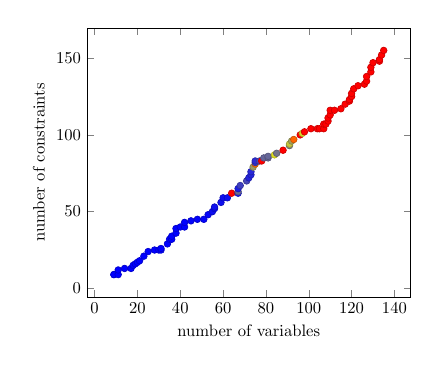
\begin{tikzpicture}[scale=0.6]
\begin{axis}[scatter, point meta=\thisrow{time}, only marks, , xlabel=number of variables,ylabel=number of constraints]

\addplot table[x=x,y=y]  { 
 x y time
 9 9 0.05 
 9 9 0.0 
 11 9 0.0 
 11 12 0.0 
 14 13 0.0 
 17 13 0.0 
 18 15 0.0 
 19 16 0.0 
 20 17 0.0 
 21 18 0.0 
 23 21 0.0 
 25 24 0.0 
 28 25 0.0 
 30 25 0.0 
 31 25 0.0 
 31 26 0.0 
 34 29 0.0 
 35 32 0.0 
 36 32 1.0 
 36 34 1.0 
 38 36 1.0 
 38 39 2.0 
 40 40 2.0 
 42 40 2.0 
 42 43 3.0 
 45 44 10.0 
 48 45 7.0 
 51 45 8.0 
 53 48 9.0 
 55 50 27.0 
 56 52 19.0 
 56 53 31.0 
 59 56 31.0 
 60 59 26.0 
 62 59 27.0 
 64 62 1440.0 
 67 62 43.0 
 67 63 199.0 
 67 65 54.0 
 68 67 118.0 
 71 70 134.0 
 72 72 68.0 
 73 74 68.0 
 73 76 76.0 
 74 79 289.0 
 75 81 1021.0 
 75 82 110.0 
 75 83 84.0 
 77 83 132.0 
 78 83 1440.0 
 79 85 190.0 
 81 85 196.0 
 81 86 194.0 
 84 87 419.0 
 85 88 218.0 
 88 90 1440.0 
 91 93 240.0 
 91 94 366.0 
 92 96 304.5 
 93 97 1056.0 
 96 100 1440.0 
 97 101 402.0 
 98 102 1440.0 
 101 104 1440.0 
 104 104 1440.0 
 105 104 1440.0 
 107 104 1440.0 
 107 107 1440.0 
 108 107 1440.0 
 109 109 1440.0 
 109 111 1440.0 
 110 113 1440.0 
 110 116 1440.0 
 112 116 1440.0 
 115 117 1440.0 
 117 120 1440.0 
 119 122 1440.0 
 119 123 1440.0 
 120 125 1440.0 
 120 127 1440.0 
 121 130 1440.0 
 123 132 1440.0 
 126 133 1440.0 
 127 135 1440.0 
 127 138 1440.0 
 129 141 1440.0 
 129 144 1440.0 
 130 147 1440.0 
 133 148 1440.0 
 133 149 1440.0 
 134 152 1440.0 
 135 155 1440.0 
};

\end{axis}
\end{tikzpicture}

\\
\tikz{\node (a) at (0.0,4) {\textsc{TheoMod}};\node (a) at (0.0,0) {};} & 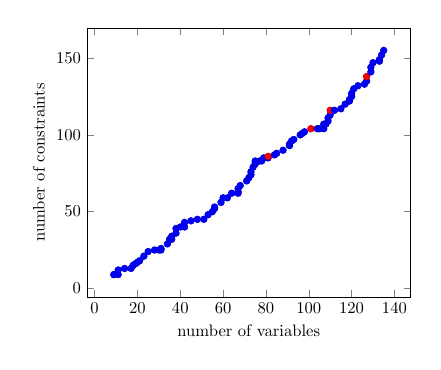
\begin{tikzpicture}[scale=0.6]
\begin{axis}[scatter, point meta=\thisrow{time}, only marks, , xlabel=number of variables,ylabel=number of constraints]

\addplot table[x=x,y=y]  { 
 x y time
 9 9 0.05 
 9 9 0.0 
 11 9 0.0 
 11 12 0.0 
 14 13 0.0 
 17 13 0.0 
 18 15 0.0 
 19 16 0.0 
 20 17 0.0 
 21 18 0.0 
 23 21 0.0 
 25 24 0.0 
 28 25 0.0 
 30 25 0.0 
 31 25 0.0 
 31 26 0.0 
 34 29 0.0 
 35 32 0.0 
 36 32 0.0 
 36 34 0.0 
 38 36 0.0 
 38 39 0.0 
 40 40 0.0 
 42 40 0.0 
 42 43 0.0 
 45 44 0.0 
 48 45 0.0 
 51 45 0.0 
 53 48 0.0 
 55 50 0.0 
 56 52 0.0 
 56 53 0.0 
 59 56 0.0 
 60 59 0.0 
 62 59 0.0 
 64 62 0.0 
 67 62 0.0 
 67 63 0.0 
 67 65 0.0 
 68 67 0.0 
 71 70 0.0 
 72 72 0.0 
 73 74 0.0 
 73 76 0.0 
 74 79 0.0 
 75 81 0.0 
 75 82 0.0 
 75 83 0.0 
 77 83 0.0 
 78 83 0.0 
 79 85 0.0 
 81 85 0.0 
 81 86 1440.0 
 84 87 0.0 
 85 88 0.0 
 88 90 0.0 
 91 93 0.0 
 91 94 0.0 
 92 96 0.5 
 93 97 0.0 
 96 100 0.0 
 97 101 0.0 
 98 102 0.0 
 101 104 1440.0 
 104 104 0.0 
 105 104 0.0 
 107 104 0.0 
 107 107 0.0 
 108 107 0.0 
 109 109 0.0 
 109 111 0.0 
 110 113 0.0 
 110 116 1440.0 
 112 116 1.0 
 115 117 1.0 
 117 120 1.0 
 119 122 1.0 
 119 123 1.0 
 120 125 1.0 
 120 127 1.0 
 121 130 1.0 
 123 132 1.0 
 126 133 1.0 
 127 135 1.0 
 127 138 1440.0 
 129 141 1.0 
 129 144 2.0 
 130 147 1.0 
 133 148 1.0 
 133 149 1.0 
 134 152 12.0 
 135 155 2.0 
};

\end{axis}
\end{tikzpicture}

 & 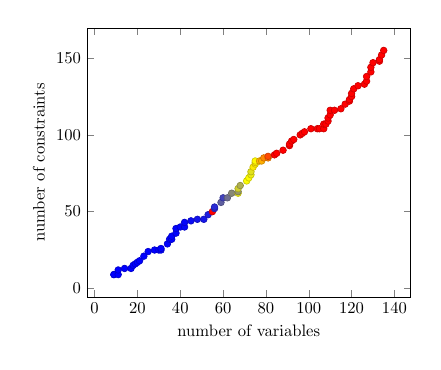
\begin{tikzpicture}[scale=0.6]
\begin{axis}[scatter, point meta=\thisrow{time}, only marks, , xlabel=number of variables,ylabel=number of constraints]

\addplot table[x=x,y=y]  { 
 x y time
 9 9 0.05 
 9 9 0.0 
 11 9 0.0 
 11 12 0.0 
 14 13 0.0 
 17 13 0.0 
 18 15 0.0 
 19 16 0.0 
 20 17 0.0 
 21 18 0.0 
 23 21 0.0 
 25 24 0.0 
 28 25 0.0 
 30 25 1.0 
 31 25 1.0 
 31 26 1.0 
 34 29 3.0 
 35 32 3.0 
 36 32 4.0 
 36 34 4.0 
 38 36 6.0 
 38 39 6.0 
 40 40 8.0 
 42 40 13.0 
 42 43 12.0 
 45 44 21.0 
 48 45 35.0 
 51 45 42.0 
 53 48 57.0 
 55 50 1440.0 
 56 52 88.0 
 56 53 79.0 
 59 56 179.0 
 60 59 124.0 
 62 59 209.0 
 64 62 257.0 
 67 62 448.0 
 67 63 283.0 
 67 65 391.0 
 68 67 326.0 
 71 70 474.0 
 72 72 484.0 
 73 74 449.0 
 73 76 425.0 
 74 79 563.0 
 75 81 539.0 
 75 82 590.0 
 75 83 496.0 
 77 83 758.0 
 78 83 781.0 
 79 85 928.0 
 81 85 936.0 
 81 86 1161.0 
 84 87 1440.0 
 85 88 1440.0 
 88 90 1440.0 
 91 93 1440.0 
 91 94 1440.0 
 92 96 1440.0 
 93 97 1440.0 
 96 100 1440.0 
 97 101 1440.0 
 98 102 1440.0 
 101 104 1440.0 
 104 104 1440.0 
 105 104 1440.0 
 107 104 1440.0 
 107 107 1440.0 
 108 107 1440.0 
 109 109 1440.0 
 109 111 1440.0 
 110 113 1440.0 
 110 116 1440.0 
 112 116 1440.0 
 115 117 1440.0 
 117 120 1440.0 
 119 122 1440.0 
 119 123 1440.0 
 120 125 1440.0 
 120 127 1440.0 
 121 130 1440.0 
 123 132 1440.0 
 126 133 1440.0 
 127 135 1440.0 
 127 138 1440.0 
 129 141 1440.0 
 129 144 1440.0 
 130 147 1440.0 
 133 148 1440.0 
 133 149 1440.0 
 134 152 1440.0 
 135 155 1440.0 
};

\end{axis}
\end{tikzpicture}

\\
\\\\
\multicolumn{3}{c}{\ref{storedcolorbar1}}\end{tabular}\end{center}

\newpage

\begin{center}\underline{\textsc{Non-Equiv + Permut} for Test of 99 small instances of knapsack}
\vspace{0.5cm}

\begin{tabular}{ccc} & gecode & coinbc\\\\\tikz{\node (a) at (0.0,4) {\textsc{QuadraMod}};\node (a) at (0.0,0) {};} & 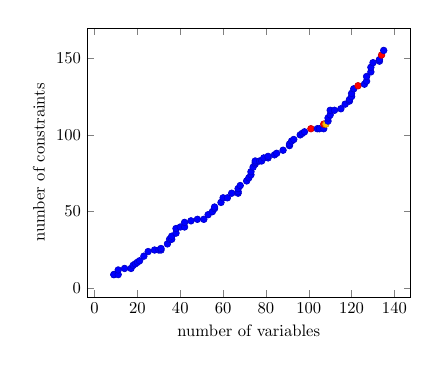
\begin{tikzpicture}[scale=0.6]
\begin{axis}[scatter, point meta=\thisrow{time}, only marks, colorbar, colorbar horizontal,colorbar style={ylabel={Time (min)}, ylabel style={rotate=270},}, colorbar to name={storedcolorbar2},, xlabel=number of variables,ylabel=number of constraints]

\addplot table[x=x,y=y]  { 
 x y time
 9 9 0.05 
 9 9 0.0 
 11 9 0.0 
 11 12 0.0 
 14 13 0.0 
 17 13 0.0 
 18 15 0.0 
 19 16 0.0 
 20 17 0.0 
 21 18 0.0 
 23 21 0.0 
 25 24 0.0 
 28 25 0.0 
 30 25 0.0 
 31 25 0.0 
 31 26 0.0 
 34 29 0.0 
 35 32 0.0 
 36 32 0.0 
 36 34 0.0 
 38 36 0.0 
 38 39 0.0 
 40 40 0.0 
 42 40 0.0 
 42 43 0.0 
 45 44 0.0 
 48 45 0.0 
 51 45 0.0 
 53 48 0.0 
 55 50 0.0 
 56 52 0.0 
 56 53 0.0 
 59 56 0.0 
 60 59 0.0 
 62 59 0.0 
 64 62 0.0 
 67 62 0.0 
 67 63 0.0 
 67 65 0.0 
 68 67 0.0 
 71 70 0.0 
 72 72 0.0 
 73 74 0.0 
 73 76 0.0 
 74 79 0.0 
 75 81 0.0 
 75 82 0.0 
 75 83 0.0 
 77 83 0.0 
 78 83 0.0 
 79 85 0.0 
 81 85 0.0 
 81 86 0.0 
 84 87 0.0 
 85 88 0.0 
 88 90 0.0 
 91 93 0.0 
 91 94 0.0 
 92 96 0.0 
 93 97 0.0 
 96 100 1.0 
 97 101 0.0 
 98 102 1.0 
 101 104 1440.0 
 104 104 0.0 
 105 104 1.0 
 107 104 1.0 
 107 107 1440.0 
 108 107 720.5 
 109 109 1.0 
 109 111 1.0 
 110 113 1.0 
 110 116 1.0 
 112 116 1.0 
 115 117 1.0 
 117 120 1.0 
 119 122 1.0 
 119 123 1.0 
 120 125 1.0 
 120 127 1.0 
 121 130 1.0 
 123 132 1440.0 
 126 133 3.0 
 127 135 3.0 
 127 138 2.0 
 129 141 2.0 
 129 144 2.0 
 130 147 2.0 
 133 148 2.0 
 133 149 2.0 
 134 152 1440.0 
 135 155 3.0 
};

\end{axis}
\end{tikzpicture}

 & 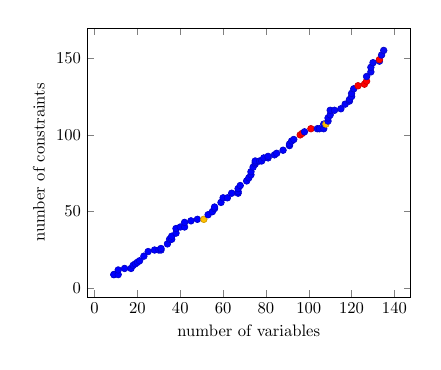
\begin{tikzpicture}[scale=0.6]
\begin{axis}[scatter, point meta=\thisrow{time}, only marks, , xlabel=number of variables,ylabel=number of constraints]

\addplot table[x=x,y=y]  { 
 x y time
 9 9 0.05 
 9 9 0.0 
 11 9 0.0 
 11 12 0.0 
 14 13 0.0 
 17 13 0.0 
 18 15 0.0 
 19 16 0.0 
 20 17 0.0 
 21 18 0.0 
 23 21 0.0 
 25 24 0.0 
 28 25 0.0 
 30 25 0.0 
 31 25 0.0 
 31 26 0.0 
 34 29 0.0 
 35 32 0.0 
 36 32 0.0 
 36 34 0.0 
 38 36 0.0 
 38 39 0.0 
 40 40 0.0 
 42 40 0.0 
 42 43 0.0 
 45 44 0.0 
 48 45 0.0 
 51 45 720.0 
 53 48 0.0 
 55 50 0.0 
 56 52 1.0 
 56 53 0.0 
 59 56 1.0 
 60 59 1.0 
 62 59 1.0 
 64 62 1.0 
 67 62 1.0 
 67 63 1.0 
 67 65 1.0 
 68 67 2.0 
 71 70 2.0 
 72 72 2.0 
 73 74 2.0 
 73 76 2.0 
 74 79 2.0 
 75 81 3.0 
 75 82 3.0 
 75 83 3.0 
 77 83 3.0 
 78 83 3.0 
 79 85 4.0 
 81 85 4.0 
 81 86 4.0 
 84 87 4.0 
 85 88 4.0 
 88 90 5.0 
 91 93 6.0 
 91 94 4.0 
 92 96 4.0 
 93 97 4.67 
 96 100 1440.0 
 97 101 1440.0 
 98 102 6.0 
 101 104 1440.0 
 104 104 7.0 
 105 104 7.0 
 107 104 7.0 
 107 107 7.0 
 108 107 723.0 
 109 109 8.0 
 109 111 7.0 
 110 113 9.0 
 110 116 7.0 
 112 116 10.0 
 115 117 8.0 
 117 120 10.0 
 119 122 11.0 
 119 123 10.0 
 120 125 9.0 
 120 127 10.0 
 121 130 10.0 
 123 132 1440.0 
 126 133 1440.0 
 127 135 1440.0 
 127 138 14.0 
 129 141 14.0 
 129 144 13.0 
 130 147 15.0 
 133 148 17.0 
 133 149 1440.0 
 134 152 16.0 
 135 155 20.0 
};

\end{axis}
\end{tikzpicture}

\\
\tikz{\node (a) at (0.0,4) {\textsc{TheoMod}};\node (a) at (0.0,0) {};} & 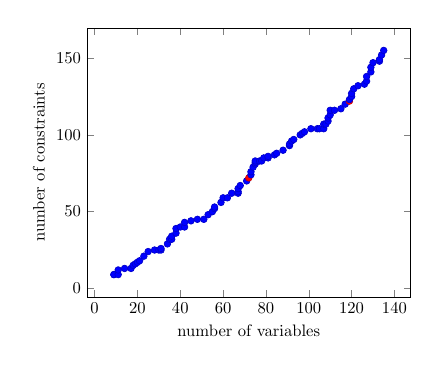
\begin{tikzpicture}[scale=0.6]
\begin{axis}[scatter, point meta=\thisrow{time}, only marks, , xlabel=number of variables,ylabel=number of constraints]

\addplot table[x=x,y=y]  { 
 x y time
 9 9 0.05 
 9 9 0.0 
 11 9 0.0 
 11 12 0.0 
 14 13 0.0 
 17 13 0.0 
 18 15 0.0 
 19 16 0.0 
 20 17 0.0 
 21 18 0.0 
 23 21 0.0 
 25 24 0.0 
 28 25 0.0 
 30 25 0.0 
 31 25 0.0 
 31 26 0.0 
 34 29 0.0 
 35 32 0.0 
 36 32 0.0 
 36 34 0.0 
 38 36 0.0 
 38 39 0.0 
 40 40 0.0 
 42 40 0.0 
 42 43 0.0 
 45 44 0.0 
 48 45 0.0 
 51 45 0.0 
 53 48 0.0 
 55 50 0.0 
 56 52 0.0 
 56 53 0.0 
 59 56 0.0 
 60 59 0.0 
 62 59 0.0 
 64 62 0.0 
 67 62 0.0 
 67 63 0.0 
 67 65 0.0 
 68 67 0.0 
 71 70 0.0 
 72 72 1440.0 
 73 74 0.0 
 73 76 0.0 
 74 79 0.0 
 75 81 0.0 
 75 82 0.0 
 75 83 0.0 
 77 83 0.0 
 78 83 0.0 
 79 85 0.0 
 81 85 0.0 
 81 86 0.0 
 84 87 0.0 
 85 88 0.0 
 88 90 0.0 
 91 93 0.0 
 91 94 0.0 
 92 96 0.0 
 93 97 0.0 
 96 100 0.0 
 97 101 0.0 
 98 102 0.0 
 101 104 0.0 
 104 104 0.0 
 105 104 0.0 
 107 104 0.0 
 107 107 0.0 
 108 107 0.0 
 109 109 0.0 
 109 111 0.0 
 110 113 0.0 
 110 116 0.0 
 112 116 0.0 
 115 117 0.0 
 117 120 0.0 
 119 122 1440.0 
 119 123 0.0 
 120 125 0.0 
 120 127 0.0 
 121 130 0.0 
 123 132 0.0 
 126 133 0.0 
 127 135 0.0 
 127 138 0.0 
 129 141 0.0 
 129 144 0.0 
 130 147 0.0 
 133 148 0.0 
 133 149 0.0 
 134 152 0.0 
 135 155 0.0 
};

\end{axis}
\end{tikzpicture}

 & 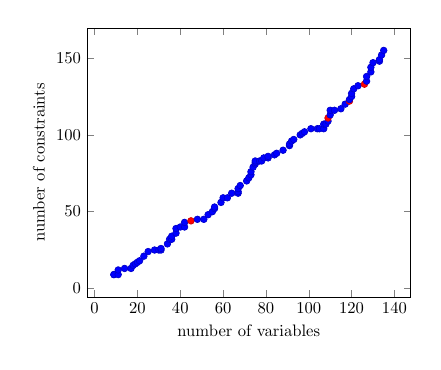
\begin{tikzpicture}[scale=0.6]
\begin{axis}[scatter, point meta=\thisrow{time}, only marks, , xlabel=number of variables,ylabel=number of constraints]

\addplot table[x=x,y=y]  { 
 x y time
 9 9 0.05 
 9 9 0.0 
 11 9 0.0 
 11 12 0.0 
 14 13 0.0 
 17 13 0.0 
 18 15 0.0 
 19 16 0.0 
 20 17 0.0 
 21 18 0.0 
 23 21 0.0 
 25 24 0.0 
 28 25 0.0 
 30 25 0.0 
 31 25 0.0 
 31 26 0.0 
 34 29 0.0 
 35 32 0.0 
 36 32 0.0 
 36 34 0.0 
 38 36 0.0 
 38 39 0.0 
 40 40 0.0 
 42 40 0.0 
 42 43 0.0 
 45 44 1440.0 
 48 45 0.0 
 51 45 0.0 
 53 48 0.0 
 55 50 0.0 
 56 52 0.0 
 56 53 0.0 
 59 56 0.0 
 60 59 0.0 
 62 59 0.0 
 64 62 0.0 
 67 62 0.0 
 67 63 0.0 
 67 65 0.0 
 68 67 0.0 
 71 70 0.0 
 72 72 0.0 
 73 74 0.0 
 73 76 0.0 
 74 79 0.0 
 75 81 0.0 
 75 82 0.0 
 75 83 0.0 
 77 83 0.0 
 78 83 0.0 
 79 85 0.0 
 81 85 0.0 
 81 86 0.0 
 84 87 0.0 
 85 88 0.0 
 88 90 0.0 
 91 93 0.0 
 91 94 0.0 
 92 96 0.0 
 93 97 0.0 
 96 100 0.0 
 97 101 0.0 
 98 102 0.0 
 101 104 0.0 
 104 104 0.0 
 105 104 0.0 
 107 104 0.0 
 107 107 0.0 
 108 107 0.0 
 109 109 0.0 
 109 111 1440.0 
 110 113 0.0 
 110 116 0.0 
 112 116 0.0 
 115 117 0.0 
 117 120 0.0 
 119 122 1440.0 
 119 123 0.0 
 120 125 0.0 
 120 127 0.0 
 121 130 0.0 
 123 132 0.0 
 126 133 1440.0 
 127 135 0.0 
 127 138 0.0 
 129 141 0.0 
 129 144 0.0 
 130 147 0.0 
 133 148 0.0 
 133 149 0.0 
 134 152 0.0 
 135 155 0.0 
};

\end{axis}
\end{tikzpicture}

\\
\\\\
\multicolumn{3}{c}{\ref{storedcolorbar2}}\end{tabular}\end{center}

\newpage

\end{document}